\documentclass[a4 paper]{article}
% Set target color model to RGB
\usepackage[inner=2.0cm,outer=2.0cm,top=2.5cm,bottom=2.5cm]{geometry}
\usepackage{setspace}
\usepackage[rgb]{xcolor}
\usepackage{verbatim}
\usepackage{subcaption}
\usepackage{amsgen,amsmath,amstext,amsbsy,amsopn,tikz,amssymb,tkz-linknodes}
\usepackage{fancyhdr}
\usepackage[colorlinks=true, urlcolor=blue,  linkcolor=blue, citecolor=blue]{hyperref}
\usepackage[colorinlistoftodos]{todonotes}
\usepackage{rotating}
\usepackage{algorithm2e}

\usepackage{listings}
\usepackage{color}
\usepackage{graphicx} 

\newcommand{\code}[1]{\texttt{#1}}

\lstset{
  tabsize=2,
  basicstyle=\fontsize{12}{5.5}\ttfamily,
  language=C,
  showspaces=false,
  showtabs=false,
  % numbers = left,
  breaklines=true,
  showstringspaces=false,
  breakatwhitespace=true,
  keywordstyle=\color[rgb]{0,0,1},
	commentstyle=\color[rgb]{0.133,0.545,0.133},
	stringstyle=\color[rgb]{0.627,0.126,0.941},
  basicstyle=\ttfamily,
  moredelim=[il][\textcolor{pgrey}]{$$},
  moredelim=[is][\textcolor{pgrey}]{\%\%}{\%\%}
}

\usepackage{booktabs}
\newcommand{\ra}[1]{\renewcommand{\arraystretch}{#1}}

\newcommand{\homework}[6]{
   \pagestyle{myheadings}
   \thispagestyle{plain}
   \newpage
  

  \pagestyle{fancy}
  \fancyhead[RO,LE]{\thepage}
  \fancyhf{} % clear all fields

  
   \setcounter{page}{1}
   \noindent
   \begin{center}
   \framebox{
      \vbox{\vspace{2mm}
    \hbox to 6.28in { {\bf COL331:~Operating Systems \hfill { #2}} }
       \vspace{6mm}
       \hbox to 6.28in { {\LARGE \hfill #1  \hfill} }
       \vspace{6mm}
       \hbox to 6.28in {\bf {Entry Number: {\rm #4} \hfill Name: {\rm #5} } }
       % \hbox to 6.28in { {\it TA: #4  \hfill #6}}
      \vspace{2mm}}
   }
   \end{center}
   \lhead{#1}
   \rhead{Page \thepage}
   % \markboth{#1}{#1}
   \cfoot{\thepage}
   \vspace*{4mm}
}

% \newcommand{\problem}[2]{~\\\fbox{\textbf{Problem #1}}\hfill (#2 points)\newline\newline}
% \newcommand{\subproblem}[1]{~\newline\textbf{(#1)}}
% \newcommand{\D}{\mathcal{D}}
% \newcommand{\Hy}{\mathcal{H}}
% \newcommand{\VS}{\textrm{VS}}
% \newcommand{\solution}{~\newline\textbf{\textit{(Solution)}} }

% \newcommand{\bbF}{\mathbb{F}}
% \newcommand{\bbX}{\mathbb{X}}
% \newcommand{\bI}{\mathbf{I}}
% \newcommand{\bX}{\mathbf{X}}
% \newcommand{\bY}{\mathbf{Y}}
% \newcommand{\bepsilon}{\boldsymbol{\epsilon}}
% \newcommand{\balpha}{\boldsymbol{\alpha}}
% \newcommand{\bbeta}{\boldsymbol{\beta}}
% \newcommand{\0}{\mathbf{0}}

\begin{document}
\homework{Assignment 1 Report}{Date: February 24, 2019}{}{\bf 2016CS10363}{\bf Manish Tanwar}{NetId(s)}


\section{Inter-Process Communication:}

\subsection*{Unicasting:}
\begin{itemize}
  \item A queue is added for each process to hold the pending messages for that process.
  \begin{lstlisting}
    struct msg_queue
    {
      struct spinlock lock;
      char data[BUFFER_SIZE][MSGSIZE];
      int start;
      int end;
      int channel; // channel is used for sleep and wakeup
    }MsgQueue[NPROC];
  \end{lstlisting}

  \item System Calls:
  \begin{lstlisting}
  int send(int sender_pid, int rec_pid, void *msg);
  int recv(void *msg);
  \end{lstlisting}
  \item Sending a Message: Syscall \code{send} enqueues the message to the receiver's message queue, it also wakeups the receiver process as it might be waiting for a message. It returns error(-1) if the queue is full.
  \item Receiving a Message: Syscall \code{recv} dequeues a message from it's message queue and stores it in \code{msg}. If the queue is empty, than the receiving process is blocked by calling \code{sleep} on a certain channel, so it's a blocking call.

\end{itemize}


\subsection*{Signal Handling:}
\begin{itemize}

% \raggedbottom\lstinputlisting[language=C]{codes/1.c}
\item \textbf{Signal Handler Function Signature:}
% \par 

\begin{lstlisting}
      typedef void (*sighandler_t)(void*);
\end{lstlisting}

\vspace*{-1.5mm}

\begin{itemize}
\item \texttt{sighandler\_t} is a function pointer which takes a void pointer as an argument and returns void.
\end{itemize}

\item \textbf{System Calls for Signal Handling:}

\raggedbottom\lstinputlisting[language=C]{codes/1.c}

\item \textbf{Added Fields in Proc Struct:}

\begin{itemize}
  \item Signal Handlers : It stores function pointers to signal handlers for that process, i.e if another process sends this process a signal with \code{sig\_num} then the Signal Handler is implemented which is pointed by the stored function pointer. Pointer is set to 0, if no signal handler is set.
  \item Signal Queue : A queue to store the pending signals for that process. It stores \code{sig\_num} and \code{sig\_arg} for each pending signal. The queue is implemented using an array with constant size 256 (circular array implementation).

  \begin{lstlisting}
    struct sig_queue
    {
      struct spinlock lock;
      char sig_arg[SIG_QUE_SIZE][MSGSIZE];
      int sig_num_list[SIG_QUE_SIZE];
      int start; // works as a channel(for sleep and wakeup) also
      int end;
    };
  \end{lstlisting}
\end{itemize}

\item \textbf{Setting a Signal Handler:}
\begin{itemize}
  \item Function Signature: \begin{lstlisting}
int sig_set(int sig_num, sighandler_t handler);
  \end{lstlisting}
  \item The system call \code{sig\_set} is called by the receiver to set the signal handler's function pointer.
  \item The system call \code{fork} copies the parent's signal handlers to child's process.
  \item The system call \code{exec} resets the signal handlers to default value 0.
  \item The function \code{allocproc} resets the \code{sig\_queue} to an empty queue.
\end{itemize}

\item \textbf{Sending a Signal:}
\begin{itemize}
  \item Function Signature: \begin{lstlisting}
int sig_send(int dest_pid, int sig_num, void *sig_arg);
  \end{lstlisting}
  \item The sender calls syscall \code{sig\_send} for sending a signal to process with pid \code{dest\_pid}.
  \item The receiver process will be implemented it's signal handler indexed with \code{sig\_num} with argument \code{sig\_arg}, only if there is a signal handler set to \code{sig\_num} by the receiver already.
\end{itemize}

\item \textbf{Handling a Signal:}
\begin{itemize}
  \item Whenever a process is about to return from kernel mode to user mode with function call \code{trepret} (implemented in trapasm.S) it checks the signal queue by calling the function \code{execute\_signal\_handler}.
  \item Function \code{execute\_signal\_handler} does the following:
  \begin{itemize}
    \item If there is no signal available for this process, then it returns back to \code{trepret}.
    \item \textbf{Setting up user stack:} (for calling the signal handler)
  
    \begin{enumerate}
      \item For saving the user mode's context, it saves the trapframe of this process from the kernel stack to the user mode stack.
      \item It changes the register \code{\%eip} (stored in the trapframe) to the function pointer of the signal handler.
      \item We can push the parameter \code{sig\_arg} on the stack, but this pointer points to an address in kernel space(which can't be accessed by the signal handler which is implemented in the user mode), so we first push 8 bytes of the message on the stack and then we push the pointer to the first byte pushed on to the stack as a pointer.
      \item Returning back to kernel mode is necessary to retrieve back the user mode context.
      \item For returning back from the user mode to kernel mode, we have to make a syscall \code{sig\_ret} but the signal handler might not call this syscall due to other interrupts. To solve this problem we wrap up the system call code(written in \code{x86} assembly) on the stack and call it implicitly by pushing the return address for signal handler as the wrapped code's first instruction.
      \item Return back to \code{trapret} function to call user mode's signal handler.
    \end{enumerate}
    
  \end{itemize}

  \item Returning from Signal Handling:
  \begin{itemize}
    \item When the signal handler executes the wrapped code on the stack, it calls \code{sig\_ret} syscall.
    \item \code{sig\_ret} syscall just save the trapfram back from user stack to the kernel stack which retrieves back the original user mode context.
  \end{itemize}
\end{itemize}

    \begin{figure}[ht!]
      \centering %width=90mm
      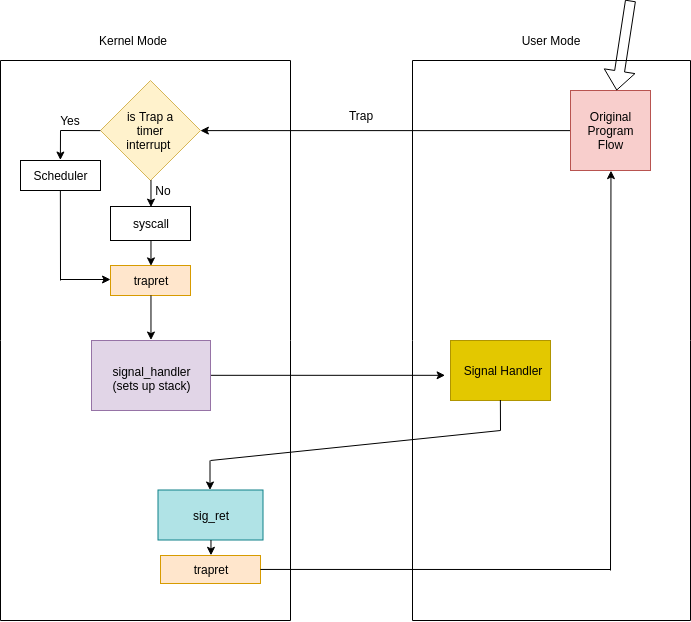
\includegraphics[width=120mm]{./Diagrams/flow_control.png}
      \caption{Flow Control of Receiver Processor on Signal Handling\label{MI1MD}}
    \end{figure}

    % \vspace*{-0.4cm\}

    \begin{figure}[ht!]
      \centering %width=90mm
      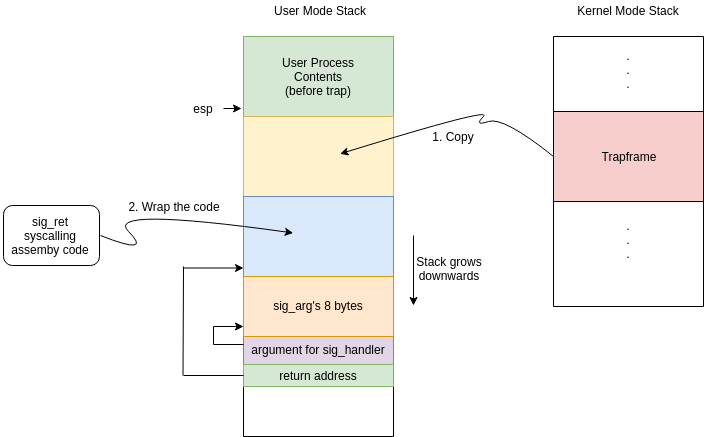
\includegraphics[width=130mm]{./Diagrams/stack_diagram.png}
      \caption{Setting up the User Stack\label{MIMD}}
    \end{figure}

  \newpage

  \item \textbf{Waiting for a Signal:}
  \begin{itemize}
    \item A process may want to wait for a signal to arrive. 
    \item A process can make \code{sig\_pause} to get blocked until a signal arrives for it.
    \item \code{sig\_pause} checks if there is any signal available for this process if there is not then it gets blocked by calling function \code{sleep} on a certain channel.
    \item Syscall \code{sig\_send} wakeups the receiver process which might be waiting for a signal. 
  \end{itemize}
\end{itemize}

\subsection*{Multicasting:}

\begin{itemize}
  \item System Call Signature:
  \begin{lstlisting}
int send_multi(int sender_pid,int rec_pids[],void *msg,int rec_length);
  \end{lstlisting}
  \vspace*{-3mm}
  \item First, all the receiver has to set their signal handler (with default \code{sig\_num} = 0) for receiving a message.
  \item Syscall \code{send\_multi} sends signals to all the receiver processes (with pid's as \code{rec\_pids[]}) with \code{sig\_num} = 0 with the argument \code{sig\_arg} = \code{msg}.
  \item Message is delivered when the receiver processes switch from kernel mode to user mode after a trap.
\end{itemize}


\section{Distributed Algorithm:}

\begin{itemize}
  \item The coordinator(parent) process forks $n$ child process(workers). $n$ is kept equal to 8 but can be scaled up. (tested up to $32$)
  \item Every worker process is assigned equal size subarrays to proceed on (with an exception of the last child process).
  \item Every worker process computes the partial sum of subarray assigned and sends it to the coordinator using unicasting function implemented.
  \item The coordinator collects the partial sums and computes the total sum. Then it multicasts the mean to each worker process.
  \item Every worker process computes the sum of the squares of the differences about the mean and sends to the coordinator using unicasting.
  \item The coordinator collects the partial square sums and computes the variance.
\end{itemize}
  
\section{Extra Works:}
\begin{itemize}
  \item Traps are not disabled during the execution of the signal handler.
  \item We can make system calls in the signal handler.
  \item Can handle nested executions of signal handlers.
  \item Support of multiple signal handlers.
  \item Implemented a syscall waiting for a signal(blocking call).
  \item The message queue is implemented efficiently.
  \item The maximum number of worker processes in the distributed algorithm can be up to 32 as well.
\end{itemize}

\end{document} 